\documentclass[11pt,a4paper]{article}

\usepackage[left=2cm, right=2cm, top=2cm, bottom=2cm]{geometry}
\usepackage{graphicx}
\usepackage{mathtools}
\usepackage{amssymb}
\usepackage{hyperref}
\usepackage{siunitx}
\usepackage[version=4]{mhchem}
\usepackage{tabularray}
\usepackage{natbib}

\title{xxx: Supporting information}
\author{Pierre Beaujean}
\begin{document}
\maketitle


\renewcommand{\thetable}{S\arabic{table}}
\renewcommand{\thefigure}{S\arabic{figure}}

\begin{figure}[!h]
	\centering
	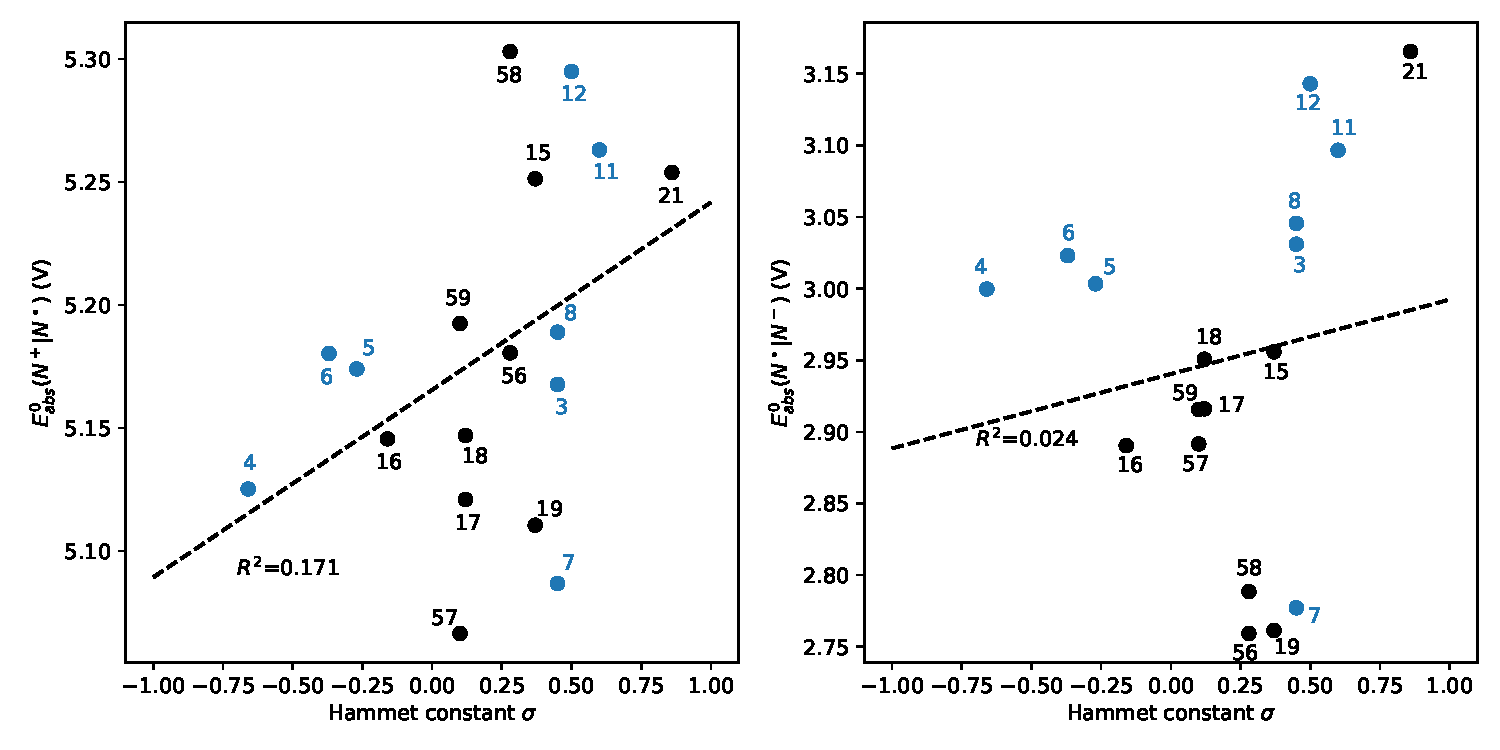
\includegraphics [width=\linewidth]{FigureS1}
	\caption{Evolution of the Born solvatation energy, $\Delta G^\star_{Born}$ (computed with Eq.~(4) of the main text) with the dielectric constant of the solvent (left) for different spherical cavities ($a$) and of the Debye-Huckel correction, $\Delta G^\star_{DH}$  (computed with Eq.~(5) of the main text) with the concentration in electrolyte, $[X]$ (right) in water and acetontrile.}
\end{figure}

\begin{figure}[!h]
\centering
\includegraphics [width=.5\linewidth]{FigureS2}
\caption{Impact of the concentration of electrolyte on the formal oxidation (plain lines, computed with Eq.~(9) of the main text) and reduction (dashed lines, computed with Eq.~(10) of the main text) potentials, $E^f_{abs}$, considering a fictitious case where $E^0_{abs} = \SI{0}{\volt}$.}
\end{figure}

\begin{figure}[!h]
\centering
\includegraphics [width=.7\linewidth]{FigureS3}
\caption{Evolution of the pairing energy, $\Delta G^\star_{pair}$ (computed with Eq.~(11) of the main text) between two ions, with the ratio between the radii of the two ions ($\chi$) and for increasing dipole cavity shapes ($s_2$). Their charge is set to 1 and -1, and two possible scaling for  the close contact distance is used ($s_1$, left and right). The equilibrium constant, $K_{pair} = e^{-\frac{\Delta G^\star_{pair}}{RT}}$, is reported. }
\end{figure}

\clearpage
\begin{longtblr}[caption={Radii ($a$, in \si{\angstrom}) for all oxidized states of compounds \textbf{1}-\textbf{61} and corresponding absolute redox potentials ($E^0_{abs}$, in \si{\volt}), as computed at the $\omega$B97X-D/6-311+G(d) level in water (SMD), with $[\ce{X}]=\SI{0}{\mole\per\liter}$.}]{colspec={>{\bfseries}lX[c]X[c]X[c]X[c]X[c]},width = 0.85\linewidth, rowhead=1}
	\hline
	& $a_{\ce{N+}}$ & $a_{\ce{N^.}}$ & $a_{\ce{N-}}$ & $E^0_{abs}(\ce{N+}|\ce{N^.})$ & $E^0_{abs}(\ce{N^.}|\ce{N-})$\\
	\hline
	01 & 3.40 & 3.38 & 3.39 & 5.00 & 2.88\\
	02 & 3.33 & 3.30 & 3.34 & 5.09 & 2.97\\
	03 & 3.92 & 3.91 & 3.90 & 5.17 & 3.03\\
	04 & 3.36 & 3.35 & 3.35 & 5.13 & 3.00\\
	05 & 3.91 & 3.91 & 3.91 & 5.18 & 3.00\\
	06 & 3.31 & 3.30 & 3.34 & 5.18 & 3.02\\
	07 & 4.27 & 4.47 & 4.46 & 5.09 & 2.77\\
	08 & 4.06 & 4.05 & 4.06 & 5.19 & 3.04\\
	09 & 4.05 & 4.04 & 4.05 & 5.29 & 3.13\\
	10 & 4.16 & 4.16 & 4.16 & 5.32 & 3.14\\
	11 & 3.37 & 3.36 & 3.36 & 5.29 & 3.10\\
	12 & 3.33 & 3.31 & 3.34 & 5.30 & 3.14\\
	13 & 3.28 & 3.30 & 3.34 & 5.14 & 2.99\\
	14 & 3.27 & 3.27 & 3.24 & 5.08 & 2.84\\
	15 & 3.57 & 3.82 & 3.74 & 5.26 & 2.95\\
	16 & 3.27 & 3.26 & 3.24 & 5.15 & 2.89\\
	17 & 3.47 & 3.48 & 3.85 & 5.13 & 2.91\\
	18 & 3.25 & 3.25 & 3.24 & 5.15 & 2.95\\
	19 & 4.20 & 4.19 & 4.33 & 5.11 & 2.76\\
	20 & 3.81 & 3.81 & 3.81 & 5.33 & 3.03\\
	21 & 3.27 & 3.24 & 3.23 & 5.28 & 3.17\\
	22 & 3.24 & 3.23 & 3.18 & 5.35 & 3.10\\
	23 & 3.60 & 3.60 & 3.62 & 5.27 & 2.96\\
	24 & 4.58 & 4.58 & 4.62 & 5.29 & 3.07\\
	25 & 4.05 & 4.02 & 4.01 & 5.23 & 2.96\\
	26 & 4.65 & 4.66 & 4.69 & 5.23 & 2.98\\
	27 & 3.94 & 3.94 & 3.98 & 5.24 & 2.99\\
	28 & 5.01 & 5.00 & 5.07 & 5.24 & 2.79\\
	29 & 4.30 & 4.29 & 4.24 & 5.28 & 3.08\\
	30 & 4.32 & 4.32 & 4.35 & 5.36 & 3.12\\
	31 & 4.61 & 4.60 & 4.62 & 5.32 & 3.12\\
	32 & 4.57 & 4.57 & 4.58 & 5.34 & 3.11\\
	33 & 4.63 & 4.64 & 4.65 & 5.34 & 3.04\\
	34 & 4.69 & 4.71 & 4.24 & 5.27 & 3.01\\
	35 & 4.05 & 4.04 & 4.07 & 5.34 & 3.06\\
	36 & 4.13 & 4.14 & 4.13 & 5.24 & 3.10\\
	37 & 4.58 & 4.62 & 4.61 & 5.26 & 3.15\\
	38 & 5.21 & 5.18 & 5.00 & 5.30 & 3.08\\
	39 & 5.10 & 5.09 & 5.11 & 5.30 & 3.15\\
	40 & 5.19 & 5.10 & 5.17 & 5.31 & 3.19\\
	41 & 5.09 & 5.05 & 5.06 & 5.29 & 3.21\\
	42 & 5.08 & 5.12 & 5.00 & 5.33 & 3.08\\
	43 & 5.47 & 5.49 & 5.68 & 5.31 & 3.15\\
	44 & 5.32 & 5.41 & 5.46 & 5.29 & 3.22\\
	45 & 5.21 & 4.90 & 4.98 & 5.31 & 3.19\\
	46 & 5.14 & 5.17 & 5.15 & 5.32 & 3.16\\
	47 & 5.22 & 5.22 & 5.55 & 5.29 & 3.13\\
	48 & 5.12 & 5.13 & 4.79 & 5.31 & 3.16\\
	49 & 4.13 & 4.14 & 4.14 & 5.14 & 3.07\\
	50 & 4.56 & 4.52 & 4.57 & 5.24 & 3.08\\
	51 & 4.52 & 4.50 & 4.49 & 5.19 & 3.06\\
	52 & 4.11 & 4.12 & 4.12 & 5.35 & 3.19\\
	53 & 4.74 & 4.71 & 4.68 & 5.36 & 3.13\\
	54 & 4.63 & 4.64 & 4.65 & 5.33 & 3.17\\
	55 & 4.67 & 4.68 & 4.67 & 5.41 & 3.23\\
	56 & 3.80 & 3.85 & 3.88 & 5.18 & 2.76\\
	57 & 3.57 & 3.54 & 3.60 & 5.07 & 2.89\\
	58 & 3.67 & 3.65 & 3.64 & 5.31 & 2.78\\
	59 & 3.63 & 3.62 & 3.65 & 5.20 & 2.91\\
	60 & 4.01 & 4.00 & 4.01 & 5.31 & 3.04\\
	\hline
\end{longtblr}

\clearpage
\begin{longtblr}[caption={Radii ($a$, in \si{\angstrom}) for all oxidized states of the compounds and corresponding absolute redox potentials ($E^0_{abs}$, in \si{\volt}), as computed at the $\omega$B97X-D/6-311+G(d) level in acetontrile (SMD), with $[\ce{X}]=\SI{0}{\mole\per\liter}$.}]{colspec={>{\bfseries}lX[c]X[c]X[c]X[c]X[c]},width = 0.85\linewidth, rowhead=1}
	\hline
	& $a_{\ce{N+}}$ & $a_{\ce{N^.}}$ & $a_{\ce{N-}}$ & $E^0_{abs}(\ce{N+}|\ce{N^.})$ & $E^0_{abs}(\ce{N^.}|\ce{N-})$\\
	\hline
	02 & 3.33 & 3.30 & 3.35 & 4.99 & 2.32\\
	03 & 3.92 & 3.91 & 3.90 & 5.15 & 2.37\\
	06 & 3.31 & 3.30 & 3.35 & 5.11 & 2.37\\
	12 & 3.33 & 3.31 & 3.34 & 5.58 & 2.45\\
	15 & 3.58 & 3.81 & 3.74 & 5.20 & 2.30\\
	23 & 3.61 & 3.60 & 3.62 & 5.24 & 2.33\\
	24 & 4.59 & 4.57 & 4.62 & 5.27 & 2.37\\
	25 & 4.05 & 4.03 & 4.02 & 5.19 & 2.30\\
	26 & 4.65 & 4.65 & 4.68 & 5.22 & 2.31\\
	27 & 3.95 & 3.94 & 3.98 & 5.23 & 2.32\\
	33 & 4.63 & 4.64 & 4.65 & 5.28 & 2.42\\
	36 & 4.13 & 4.12 & 4.08 & 5.19 & 2.51\\
	51 & 4.53 & 4.50 & 4.47 & 5.12 & 2.47\\
	54 & 4.61 & 4.62 & 4.63 & 5.33 & 2.58\\
	55 & 4.68 & 4.68 & 4.62 & 5.40 & 2.68\\
	58 & 3.66 & 3.65 & 3.64 & 5.24 & 2.12\\
	59 & 3.62 & 3.61 & 3.65 & 5.14 & 2.27\\
	60 & 4.01 & 3.99 & 4.02 & 5.28 & 2.36\\
	\hline
\end{longtblr}

\clearpage

\begin{figure}[!h]
	\centering
	\includegraphics [width=\linewidth]{FigureS4}
	\caption{Correlation between absolute oxidation (left) and reduction (right) and the Hammet constant of their substituent for compounds of the P5O (black markers) and P6O (blue markers) families.}
\end{figure}

\clearpage

\begin{longtblr}[caption={Distance ($r$, in \si{\angstrom}), $x$-component of the dipole moment  ($\mu_x$, in \si{\elementarycharge\bohr}) and $xx$ component of the traceless quadrupole moment  ($Q_{xx}$, in \si{\elementarycharge\bohr\squared}) for all compounds, as computed at the $\omega$B97X-D/6-311+G(d) level in gas phase for model geometries ($>$\ce{N-O^.} replaced by \ce{CH2}, see main text) }]{colspec={>{\bfseries}lX[c]X[c]X[c]}, width = 0.85\linewidth, rowhead=1}
	\hline
	& $r$ & $\mu_x$ & $Q_{xx}$\\
	\hline
	02 & 2.87 & -0.05 & -0.06\\
	03 & 2.87 & 0.29 & 3.36\\
	04 & 2.89 & 0.33 & -1.26\\
	05 & 2.87 & 0.19 & 0.99\\
	06 & 2.87 & 0.73 & -2.41\\
	07 & 2.86 & 0.35 & 3.14\\
	08 & 2.86 & 0.29 & 1.94\\
	09 & 2.86 & 0.63 & 3.10\\
	10 & 2.85 & 0.80 & -0.49\\
	12 & 2.83 & 1.28 & -1.44\\
	13 & 2.80 & 0.06 & 0.64\\
	14 & 2.20 & -0.02 & -0.03\\
	15 & 2.20 & 0.29 & 2.22\\
	16 & 2.20 & 0.42 & -2.33\\
	17 & 2.21 & -0.33 & 1.09\\
	18 & 2.21 & -0.03 & 0.10\\
	19 & 2.20 & 0.34 & 1.26\\
	20 & 2.19 & 0.77 & 0.35\\
	22 & 2.15 & 0.62 & -0.24\\
	23 & 2.19 & 0.17 & 2.74\\
	24 & 2.19 & 0.61 & 7.84\\
	25 & 2.19 & -0.27 & 2.42\\
	26 & 2.19 & 0.18 & 1.13\\
	27 & 2.19 & 0.03 & 3.80\\
	28 & 2.18 & 0.60 & 7.36\\
	29 & 2.19 & -0.01 & 4.95\\
	30 & 2.18 & -0.36 & 3.30\\
	31 & 2.18 & -0.11 & 11.49\\
	32 & 2.19 & 0.70 & 5.41\\
	33 & 2.18 & 1.14 & 6.51\\
	34 & 2.19 & -0.22 & 5.34\\
	36 & 2.81 & 0.26 & 4.61\\
	37 & 2.81 & 0.31 & 5.55\\
	38 & 2.82 & 0.50 & 9.83\\
	39 & 2.83 & 0.77 & 8.60\\
	40 & 2.81 & 0.68 & 7.29\\
	41 & 2.81 & 0.45 & 12.13\\
	42 & 2.82 & 0.96 & 5.67\\
	43 & 2.81 & -0.43 & 1.02\\
	44 & 2.81 & -0.07 & 5.29\\
	45 & 2.82 & 1.42 & 4.35\\
	46 & 2.83 & 0.25 & 10.50\\
	47 & 2.81 & -0.17 & 7.36\\
	48 & 2.82 & 1.19 & 10.49\\
	49 & 2.79 & -0.21 & 4.30\\
	50 & 2.82 & -0.15 & 4.82\\
	51 & 2.82 & -0.16 & 4.23\\
	52 & 2.81 & 1.01 & 7.74\\
	53 & 2.82 & 2.18 & 3.27\\
	54 & 2.83 & 2.37 & 2.41\\
	55 & 2.83 & 3.96 & 6.84\\
	56 & 2.22 & -0.19 & 2.94\\
	57 & 2.21 & 0.36 & -3.39\\
	58 & 2.19 & 0.28 & 2.91\\
	59 & 2.19 & -0.15 & 2.12\\
	60 & 2.19 & 0.98 & 2.98\\
	\hline
\end{longtblr}

\clearpage

\begin{longtblr}[caption={Radii ($a$, in \si{\angstrom}) for the ion-pair between the oxidized (\ce{N+}) or reduced (\ce{N-}) and a counterion (\ce{A-} and \ce{C+}, respectivelly) and corresponding free Gibbs energy of complexation ($\Delta G^\star_{cplx}$, in \si{\kilo\joule\per\mole}), as computed at the $\omega$B97X-D/6-311+G(d) level in water (SMD), with $[\ce{X}]=\SI{1}{\mole\per\liter}$.}]{colspec={>{\bfseries}lX[c]X[c]cX[c]X[c]}, width = 0.85\linewidth,rowhead=2}
	\hline
	&  \SetCell[c=2]{c} \ce{N+ + A- <=> NA} & & & \SetCell[c=2]{c} \ce{N- + C+ <=> CA} & \\ 
	\cline{2-3} \cline{5-6}
	& $a_{\ce{NA}}$ & $\Delta{G}_{cplx}^\star$ & & $a_{\ce{NC}}$ & $\Delta{G}_{cplx}^\star$\\
	\hline
	01 & 3.95 & 25.1 &  & 4.96 & 30.0\\
	02 & 4.45 & 23.3 &  & 4.87 & 49.7\\
	03 & 5.46 & 23.2 &  & 4.90 & 49.0\\
	04 & 4.85 & 21.0 &  & 4.96 & 48.9\\
	05 & 5.47 & 17.5 &  & 4.96 & 42.0\\
	06 & 4.97 & 23.4 &  & 4.96 & 48.6\\
	07 & 5.72 & 24.8 &  & 5.47 & 42.0\\
	08 & 4.76 & 24.6 &  & 5.24 & 51.3\\
	09 & 5.53 & 25.9 &  & 6.00 & 64.2\\
	10 & 4.72 & 28.1 &  & 5.08 & 49.7\\
	12 & 3.75 & 22.7 &  & 4.89 & 39.3\\
	13 & 3.81 & 24.1 &  & 5.13 & 24.3\\
	14 & 4.07 & 25.7 &  & 4.90 & 27.5\\
	15 & 4.99 & 29.1 &  & 5.64 & 27.0\\
	16 & 4.39 & 27.7 &  & 4.92 & 41.1\\
	17 & 5.17 & 21.6 &  & 4.88 & 32.0\\
	18 & 4.23 & 23.8 &  & 4.91 & 38.3\\
	19 & 4.97 & 39.8 &  & 5.26 & 26.4\\
	20 & 4.58 & 57.0 &  & 5.86 & 47.2\\
	21 & 4.48 & 29.7 &  & 5.32 & 21.6\\
	22 & 3.97 & 24.8 &  & 4.87 & 28.0\\
	23 & 4.52 & 21.2 &  & 6.24 & 29.9\\
	24 & 6.12 & 22.7 &  & 6.30 & 28.7\\
	25 & 4.62 & 21.9 &  & 5.73 & 27.4\\
	26 & 4.79 & 27.3 &  & 6.31 & 25.7\\
	27 & 4.58 & 23.5 &  & 5.55 & 27.3\\
	28 & 6.34 & 17.7 &  & 5.76 & 22.8\\
	29 & 4.31 & 19.2 &  & 5.71 & 31.3\\
	30 & 4.32 & 14.0 &  & 6.19 & 32.4\\
	31 & 5.83 & 24.8 &  & 6.05 & 31.5\\
	32 & 5.52 & 29.8 &  & 7.16 & 33.4\\
	33 & 5.08 & 24.7 &  & 5.63 & 26.6\\
	34 & 4.70 & 22.5 &  & 6.50 & 28.4\\
	35 & 4.28 & 21.0 &  & 5.90 & 27.0\\
	36 & 5.49 & 23.5 &  & 4.52 & 14.5\\
	37 & 5.58 & 25.4 &  & 4.57 & 16.4\\
	38 & 5.88 & 18.9 &  & 6.65 & 23.1\\
	39 & 6.57 & 21.3 &  & 6.60 & 27.4\\
	40 & 6.23 & 19.6 &  & 5.77 & 25.4\\
	41 & 6.62 & 22.0 &  & 5.03 & 20.8\\
	42 & 6.47 & 24.8 &  & 6.28 & 23.3\\
	43 & 5.85 & 20.9 &  & 5.58 & 15.7\\
	44 & 5.56 & 23.9 &  & 5.51 & 29.1\\
	45 & 6.61 & 20.6 &  & 7.27 & 32.8\\
	46 & 6.44 & 22.7 &  & 7.43 & 30.8\\
	47 & 5.91 & 25.7 &  & 5.87 & 24.8\\
	48 & 6.19 & 38.0 &  & 5.01 & 25.6\\
	50 & 5.60 & 20.6 &  & 6.53 & 27.2\\
	51 & 5.84 & 25.0 &  & 6.45 & 29.0\\
	52 & 5.61 & 25.7 &  & 4.55 & 12.6\\
	53 & 5.71 & 18.1 &  & 6.48 & 29.3\\
	54 & 5.99 & 22.9 &  & 4.70 & 16.6\\
	55 & 6.02 & 20.3 &  & 6.80 & 28.7\\
	56 & 5.26 & 20.5 &  & 5.29 & -3.9\\
	57 & 5.26 & 20.9 &  & 5.80 & 13.8\\
	58 & 5.27 & 25.8 &  & 5.05 & 8.5\\
	59 & 5.14 & 27.4 &  & 5.27 & 26.0\\
	60 & 4.22 & 22.4 &  & 5.74 & 27.8\\
	\hline
\end{longtblr}

\clearpage
\begin{longtblr}[caption={Radii ($a$, in \si{\angstrom}) for the ion-pair between the oxidized (\ce{N+}) or reduced (\ce{N-}) and a counterion (\ce{A-} and \ce{C+}, respectivelly) and corresponding free Gibbs energy of complexation ($\Delta G^\star_{cplx}$, in \si{\kilo\joule\per\mole}), as computed at the $\omega$B97X-D/6-311+G(d) level in acetonitrile (SMD), with $[\ce{X}]=\SI{1}{\mole\per\liter}$.}]{colspec={>{\bfseries}lX[c]X[c]cX[c]X[c]}, width = 0.85\linewidth,rowhead=2}
	\hline
	&  \SetCell[c=2]{c} \ce{N+ + A- <=> NA} & & & \SetCell[c=2]{c} \ce{N- + C+ <=> CA} & \\ 
	\cline{2-3} \cline{5-6}
	& $a_{\ce{NA}}$ & $\Delta{G}_{cplx}^\star$ & & $a_{\ce{NC}}$ & $\Delta{G}_{cplx}^\star$\\
	\hline
	02 & 3.82 & 27.9 &  & 4.71 & 32.0\\
	03 & 3.95 & 26.3 &  & 4.64 & 29.4\\
	06 & 3.79 & 25.3 &  & 4.64 & 30.7\\
	12 & 3.76 & -6.6 &  & 4.73 & 18.3\\
	15 & 5.08 & 33.6 &  & 5.33 & 17.6\\
	23 & 4.53 & 28.1 &  & 5.56 & 5.1\\
	25 & 4.92 & 26.2 &  & 6.32 & 14.6\\
	26 & 4.83 & 28.7 &  & 6.90 & 15.1\\
	27 & 4.49 & 27.1 &  & 6.00 & 14.1\\
	33 & 5.10 & 32.1 &  & 4.79 & 37.2\\
	36 & 5.44 & 26.8 &  & 5.80 & 9.6\\
	51 & 5.85 & 30.1 &  & 6.06 & 8.5\\
	54 & 5.97 & 18.6 &  & 6.38 & 11.7\\
	55 & 6.01 & 23.5 &  & 6.38 & 11.7\\
	58 & 5.65 & 27.2 &  & 5.66 & -7.5\\
	59 & 5.64 & 31.3 &  & 5.77 & 14.3\\
	60 & 4.30 & 27.1 &  & 6.20 & 13.9\\
	\hline
\end{longtblr}

\begin{figure}[!h]
\centering
\includegraphics [width=\linewidth]{FigureS5}
\caption{Value of the complexation free Gibs energy change for $K_{01}$ (round markers, $\bullet$) and $K_{21}$ (square markers, $\blacksquare$), as computed at the $\omega$B97X-D/6-311+G(d) level in water (top) and acetonitrile (bottom) using SMD at two concentration: $[X]=\SI{1}{\mole\per\liter}$ (filled markers) and  $[X]=\SI{0.1}{\mole\per\liter}$ (empty markers). }
\end{figure}

\clearpage
\begin{longtblr}[caption={Radii ($a$, in \si{\angstrom}) for the ion-pair between the 3 oxidation states of the compounds and the \ce{AC} pair, tohether with their corresponding free Gibbs energy of complexation ($\Delta G^\star_{cplx}$, in \si{\kilo\joule\per\mole}), as computed at the $\omega$B97X-D/6-311+G(d) level in water (SMD), with $[\ce{X}]=\SI{1}{\mole\per\liter}$.}]{colspec={>{\bfseries}lX[c]X[c]cX[c]X[c]cX[c]X[c]}, width = 0.85\linewidth,rowhead=2}
	\hline
	&  \SetCell[c=2]{c} \ce{N+ + A- + C+ <=> NAC+} & & & \SetCell[c=2]{c} \ce{N^. + A- + C+ <=> NAC^.} & & & \SetCell[c=2]{c} \ce{N- + A- + C+ <=> NAC-}  & \\ 
	\cline{2-3} \cline{5-6} \cline{8-9}
	& $a_{\ce{NAC+}}$ & $\Delta{G}_{cplx}^\star$ &  & $a_{\ce{NAC^.}}$ & $\Delta{G}_{cplx}^\star$ &  & $a_{\ce{NAC-}}$ & $\Delta{G}_{cplx}^\star$\\
	\hline
	01 & 4.77 & 47.7 &  & 4.73 & 50.9 &  & 5.40 & 50.7\\
	02 & 5.39 & 51.8 &  & 4.89 & 50.0 &  & 6.59 & 80.6\\
	03 & 6.31 & 50.8 &  & 5.10 & 47.7 &  & 5.39 & 78.9\\
	04 & 5.67 & 48.8 &  & 4.78 & 52.9 &  & 5.06 & 66.3\\
	05 & 6.21 & 52.1 &  & 6.00 & 57.9 &  & 4.90 & 65.4\\
	06 & 5.68 & 55.5 &  & 6.04 & 51.8 &  & 5.10 & 68.0\\
	07 & 6.11 & 48.9 &  & 5.57 & 49.7 &  & 5.77 & 74.5\\
	08 & 5.24 & 52.2 &  & 4.87 & 43.3 &  & 5.38 & 70.6\\
	09 & 5.51 & 46.6 &  & 7.07 & 70.2 &  & 5.86 & 89.2\\
	10 & 5.40 & 44.8 &  & 5.13 & 46.3 &  & 6.13 & 72.2\\
	11 & 6.21 & 48.4 &  & 5.94 & 46.7 &  & 6.05 & 72.9\\
	12 & 5.65 & 55.0 &  & 4.73 & 47.2 &  & 6.21 & 68.9\\
	13 & 5.26 & 50.8 &  & 5.13 & 47.5 &  & 5.17 & 50.0\\
	14 & 5.41 & 52.7 &  & 4.67 & 52.0 &  & 4.96 & 54.1\\
	15 & 5.10 & 52.0 &  & 5.36 & 62.9 &  & 5.12 & 58.4\\
	16 & 4.97 & 50.8 &  & 6.19 & 67.8 &  & 5.97 & 59.7\\
	17 & 5.51 & 50.7 &  & 5.51 & 50.8 &  & 5.10 & 56.8\\
	18 & 4.92 & 49.3 &  & 4.99 & 44.9 &  & 4.94 & 62.4\\
	19 & 5.30 & 60.1 &  & 5.94 & 67.1 &  & 5.73 & 73.6\\
	20 & 5.65 & 87.6 &  & 5.36 & 79.7 &  & 5.71 & 61.8\\
	21 & 4.68 & 50.6 &  & 4.54 & 41.2 &  & 5.14 & 43.2\\
	22 & 4.67 & 51.6 &  & 4.61 & 54.4 &  & 4.87 & 50.6\\
	23 & 5.90 & 55.3 &  & 6.13 & 55.5 &  & 6.01 & 53.9\\
	24 & 6.45 & 55.2 &  & 6.54 & 53.4 &  & 6.56 & 52.4\\
	25 & 6.57 & 49.8 &  & 5.77 & 47.9 &  & 6.21 & 52.2\\
	26 & 6.47 & 62.6 &  & 6.86 & 57.2 &  & 6.74 & 50.8\\
	27 & 5.95 & 49.5 &  & 5.66 & 54.6 &  & 5.89 & 46.5\\
	28 & 6.52 & 49.7 &  & 6.87 & 48.3 &  & 7.09 & 44.6\\
	29 & 6.35 & 51.0 &  & 6.55 & 46.7 &  & 5.92 & 59.6\\
	30 & 6.06 & 49.7 &  & 6.17 & 46.6 &  & 5.94 & 60.3\\
	31 & 6.11 & 50.7 &  & 5.92 & 41.7 &  & 6.13 & 47.4\\
	32 & 6.60 & 57.2 &  & 6.64 & 56.7 &  & 6.63 & 51.2\\
	33 & 6.47 & 55.8 &  & 6.31 & 53.5 &  & 6.47 & 45.2\\
	34 & 6.56 & 45.1 &  & 6.51 & 56.8 &  & 6.77 & 54.1\\
	35 & 6.51 & 49.3 &  & 5.89 & 50.3 &  & 6.11 & 50.2\\
	36 & 6.35 & 50.0 &  & 6.12 & 46.7 &  & 6.03 & 52.3\\
	37 & 5.60 & 51.0 &  & 5.70 & 44.7 &  & 6.51 & 41.5\\
	38 & 6.24 & 49.1 &  & 6.31 & 54.1 &  & 6.45 & 45.1\\
	39 & 6.84 & 48.4 &  & 7.03 & 51.1 &  & 7.25 & 54.9\\
	40 & 7.00 & 43.4 &  & 6.81 & 52.7 &  & 6.59 & 59.5\\
	41 & 6.60 & 48.5 &  & 7.20 & 47.4 &  & 6.69 & 54.1\\
	43 & 5.87 & 47.3 &  & 5.97 & 43.0 &  & 7.24 & 53.3\\
	44 & 5.75 & 45.8 &  & 6.08 & 35.9 &  & 6.96 & 41.9\\
	45 & 6.99 & 46.6 &  & 6.97 & 49.9 &  & 7.17 & 55.0\\
	46 & 7.22 & 50.5 &  & 7.11 & 62.0 &  & 7.22 & 55.1\\
	47 & 6.36 & 49.0 &  & 6.62 & 49.5 &  & 6.46 & 34.4\\
	48 & 6.27 & 50.6 &  & 6.22 & 59.0 &  & 6.73 & 60.8\\
	49 & 6.04 & 42.8 &  & 6.01 & 48.3 &  & 5.55 & 40.1\\
	50 & 6.47 & 51.1 &  & 6.53 & 46.9 &  & 6.27 & 48.0\\
	51 & 6.06 & 48.4 &  & 6.02 & 52.2 &  & 6.46 & 55.8\\
	52 & 5.60 & 37.0 &  & 5.96 & 51.3 &  & 6.38 & 47.5\\
	53 & 6.58 & 47.0 &  & 6.61 & 49.7 &  & 6.51 & 52.7\\
	54 & 6.01 & 48.4 &  & 6.68 & 48.2 &  & 6.82 & 54.6\\
	55 & 6.64 & 44.9 &  & 6.63 & 45.5 &  & 7.03 & 51.9\\
	56 & 5.51 & 46.4 &  & 5.61 & 51.8 &  & 5.80 & 28.9\\
	57 & 5.90 & 51.9 &  & 4.67 & 39.9 &  & 5.72 & 41.2\\
	58 & 6.14 & 51.3 &  & 5.66 & 49.9 &  & 6.35 & 34.9\\
	59 & 6.17 & 56.0 &  & 5.66 & 51.8 &  & 6.16 & 52.9\\
	60 & 6.11 & 53.1 &  & 5.72 & 55.4 &  & 6.19 & 50.7\\
	\hline
\end{longtblr}

\clearpage
\begin{longtblr}[caption={Radii ($a$, in \si{\angstrom}) for the ion-pair between the 3 oxidation states of the compounds and the \ce{AC} pair, tohether with their corresponding free Gibbs energy of complexation ($\Delta G^\star_{cplx}$, in \si{\kilo\joule\per\mole}), as computed at the $\omega$B97X-D/6-311+G(d) level in acetonitrile (SMD), with $[\ce{X}]=\SI{1}{\mole\per\liter}$.}]{colspec={>{\bfseries}lX[c]X[c]cX[c]X[c]cX[c]X[c]}, width = 0.85\linewidth,rowhead=2}
	\hline
	&  \SetCell[c=2]{c} \ce{N+ + A- + C+ <=> NAC+} & & & \SetCell[c=2]{c} \ce{N^. + A- + C+ <=> NAC^.} & & & \SetCell[c=2]{c} \ce{N- + A- + C+ <=> NAC-}  & \\ 
	\cline{2-3} \cline{5-6} \cline{8-9}
	& $a_{\ce{NAC+}}$ & $\Delta{G}_{cplx}^\star$ &  & $a_{\ce{NAC^.}}$ & $\Delta{G}_{cplx}^\star$ &  & $a_{\ce{NAC-}}$ & $\Delta{G}_{cplx}^\star$\\
	\hline
	02 & 5.53 & 70.2 &  & 4.99 & 65.9 &  & 6.07 & 62.3\\
	03 & 6.35 & 65.4 &  & 5.39 & 67.3 &  & 5.45 & 71.9\\
	06 & 5.84 & 70.3 &  & 4.73 & 49.2 &  & 4.74 & 58.9\\
	12 & 5.71 & 36.5 &  & 4.90 & 56.9 &  & 4.95 & 42.0\\
	15 & 5.08 & 74.5 &  & 5.25 & 69.6 &  & 5.10 & 50.1\\
	23 & 5.84 & 65.6 &  & 6.43 & 69.7 &  & 5.84 & 43.1\\
	24 & 6.37 & 66.8 &  & 6.74 & 65.9 &  & 6.60 & 46.9\\
	25 & 6.63 & 65.9 &  & 5.85 & 59.8 &  & 6.27 & 42.4\\
	26 & 6.28 & 73.4 &  & 6.89 & 65.0 &  & 6.87 & 41.7\\
	27 & 5.95 & 62.7 &  & 5.90 & 65.9 &  & 5.93 & 41.1\\
	33 & 6.47 & 72.5 &  & 6.22 & 62.3 &  & 6.54 & 45.0\\
	36 & 6.41 & 67.4 &  & 6.36 & 58.9 &  & 6.33 & 39.2\\
	51 & 6.37 & 56.1 &  & 6.22 & 60.3 &  & 6.74 & 37.5\\
	54 & 6.01 & 63.6 &  & 6.78 & 62.9 &  & 6.74 & 46.7\\
	55 & 6.68 & 64.4 &  & 6.78 & 60.8 &  & 6.85 & 42.4\\
	58 & 6.16 & 67.8 &  & 5.67 & 61.9 &  & 6.47 & 15.4\\
	59 & 6.23 & 66.3 &  & 5.73 & 64.4 &  & 6.16 & 57.4\\
	60 & 6.17 & 69.9 &  & 6.20 & 71.0 &  & 6.15 & 39.1\\
	\hline
\end{longtblr}


\clearpage
\begin{longtblr}[caption={Experimental $E^0_{rel}(\ce{N+}|\ce{N^.})$ (in \si{\milli\volt} vs SHE) found in the litterature for some compounds, measured in water and acetonitrile. When there are two values reported, the first one is used in the text.},
		note{a} = {From Ref.~\citenum{goldsteinStructureActivityRelationship2006}.},
		note{b} = {From Ref.~\citenum{morrisChemicalElectrochemicalReduction1991}, converted from SCE to SHE with +\SI{244}{\milli\volt} \cite{pavlishchukConversionConstantsRedox2000}.},
		note{c}={From Ref.~\citenum{blincoExperimentalTheoreticalStudies2008}.},
		note{d}={From Ref.~\citenum{zhangEffectHeteroatomFunctionality2018}, converted from Fc to SHE with +\SI{624}{\milli\volt} \cite{pavlishchukConversionConstantsRedox2000}.}
	]{colspec={>{\bfseries}lX[c]X[c]c>{\bfseries}lX[c]X[c]}, width = 0.85\linewidth,rowhead=1}
	\hline
	& Water & Acetonitrile  & & & Water & Acetonitrile\\
	\hline
		2 & 740\TblrNote{a} & 850\TblrNote{c}, 858\TblrNote{d} &  & 33 & --- & 1123\TblrNote{c} \\
		3 & 805\TblrNote{a}, 774\TblrNote{b} & 924\TblrNote{c}, 939\TblrNote{d} &  & 36 & --- & 1010\TblrNote{c} \\
		4 & 817\TblrNote{a}, 874\TblrNote{b} & 1063\TblrNote{c} &  & 51 & --- & 1102\TblrNote{c} \\
		6 & 825\TblrNote{a}, 724\TblrNote{b} & 877\TblrNote{c}, 908\TblrNote{d} &  & 54 & --- & 1096\TblrNote{c} \\
		11 & 892\TblrNote{a} & --- &  & 55 & --- & 1175\TblrNote{c} \\
		12 & 918\TblrNote{a}, 914\TblrNote{b} & 1034\TblrNote{d} &  & 56 & 867\TblrNote{a}, 874\TblrNote{b} & --- \\
		13 & 795\TblrNote{a} & --- &  & 57 & 853\TblrNote{a} & --- \\
		15 & 870\TblrNote{a}, 784\TblrNote{b} & 976\TblrNote{c} &  & 58 & 955\TblrNote{a}, 974\TblrNote{b} & 1073\TblrNote{d} \\
		18 & 814\TblrNote{b} & --- &  & 59 & --- & 1109\TblrNote{d} \\
		23 & --- & 1045\TblrNote{c} &  & 60 & --- & 1099\TblrNote{c} \\
		24 & --- & 1095\TblrNote{c} &  & 61 & --- & 996\TblrNote{d} \\
		25 & --- & 990\TblrNote{c} &   \\
		26 & --- & 1030\TblrNote{c} & \\
		27 & --- & 1023\TblrNote{c} &  &  &  &  \\
	\hline
\end{longtblr}

\clearpage


\bibliographystyle{unsrt} 
\bibliography{biblio}
	
\end{document}